\documentclass{article}
\usepackage{tikz, comment}
\usepackage{pifont}
\usepackage{fontspec}
\usetikzlibrary{arrows, decorations.markings, decorations.pathreplacing}
\begin{comment}
:Title: Not defined yet
:Tags: adjugate, classical adjoint;arc of a circle;standard position;standard form for the equation of a line, general form for the equation of a line ;transformations
:Prob: 0.071;0.0611;0.0563;0.0544;0.054
:Author: Prof.Hu Ji-shan, HKUST
:Slug: No name yet

Description Here.........
\end{comment}
\begin{document}\centering

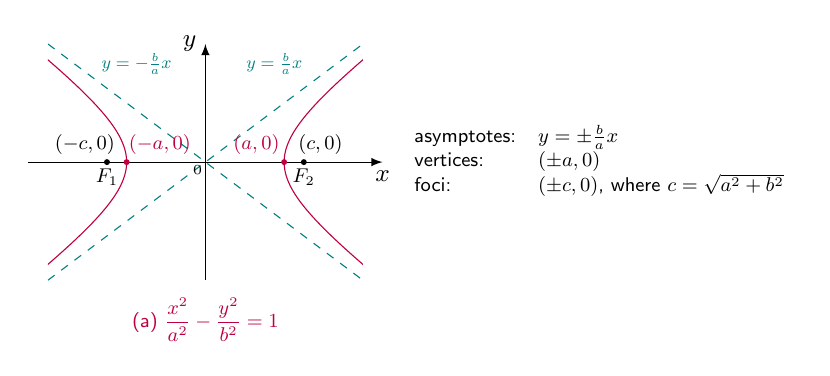
\begin{tikzpicture}[>=latex,xscale=.5*0.5, yscale=.5*0.5][font=\sf\small]

\draw[->] (-9, 0) -- (9, 0)node[below] {\small $x$};
\draw[->] (0, -6) -- (0, 6)node[left] {\small $y$};

\node[purple, scale=0.8] at (0, -8) {(a) $\displaystyle \frac{x^2}{a^2}-\frac{y^2}{b^2}=1$};

\node[scale=0.8] at (20, 0) {$
\begin{array}{ll}
\hbox{asymptotes:} & y = \pm \frac{b}{a}x \\
\hbox{vertices:} & (\pm a, 0) \\
\hbox{foci:} & \hbox{$(\pm c, 0)$, where $c = \sqrt{a^2+b^2}$}
\end{array}
$};

\clip[] (-8,-6) rectangle (8,6);

\draw[teal, dashed, samples=100, smooth, domain=-8:8, variable=\x]
plot ({\x}, {-3/4*(\x)});
\draw[teal, dashed, samples=100, smooth, domain=-8:8, variable=\x]
plot ({\x}, { 3/4*(\x)});
\node[teal, scale=0.7] at (-3.5, 5) {$y = -\frac{b}{a}x$};
\node[teal, scale=0.7] at ( 3.5, 5) {$y = \frac{b}{a}x$};

\draw[purple, samples=100, smooth, domain=-2:2, variable=\t]
plot ({4*cosh(\t)}, {3*sinh(\t)}) ;

\draw[purple, samples=100, smooth, domain=-3:3, variable=\t]
plot ({-4*cosh(\t)}, {3*sinh(\t)}) ;

\draw[fill, xscale=1/0.5, yscale=1/0.5] (-5*0.5, 0) circle(0.06) node[below, scale=0.8]{$F_1$} node[above, xshift=-8, scale=0.8]{$(-c, 0)$};
\draw[fill, xscale=1/0.5, yscale=1/0.5] ( 5*0.5, 0) circle(0.06) node[below, scale=0.8]{$F_2$} node[above, xshift= 6, scale=0.8]{$( c, 0)$};

\draw[purple, fill, xscale=1/0.5, yscale=1/0.5] (4*0.5, 0) circle(0.06) node[above, xshift=-10, scale=0.8]{$( a, 0)$};
\draw[purple, fill, xscale=1/0.5, yscale=1/0.5] (-4*0.5, 0) circle(0.06) node[above, xshift=12, scale=0.8]{$(-a, 0)$};

\node at (-0.2/0.5, -0.2/0.5) {\tiny$0$};

\end{tikzpicture}
\end{document}